\section{Autoinduzione e mutua induzione}
Fino ad ora abbiamo generato una fem grazie ad un campo magnetico
esterno che interagiva con la bobina.


Adesso proviamo a fare una fem con la corrente
che gira nel filo del solenoide.

Se si usa una corrente costante, il campo (per binot e savart)
è costante.

Se si usa una corrente variabile, anche il campo sarà variabile.


Con una \textbf{condizione di correnti stazionarie}, possiamo assumere che
La fem autoindotta è:
\begin{equation*}
    \epsilon_L = -L\frac{di}{dt}
\end{equation*}

La fem autoindotta dipende dalla velocità di variazione della corrente.

\subsection{Induttanza}
$L$ è l'induttanza di una bobina, si misura in Henry$[H] = [1VsA^{-1}]$.


La fem indotta in una bobina di N spire è:
\begin{equation}
    \epsilon_L = N\frac{d\phi_B}{dt} = -L\frac{di}{dt}
\end{equation}

\subsection{Induttanza di un lungo solenoide}
Induttanza di un lungo solenoide con spire fitte:
\begin{itemize}
    \item l = lunghezza
    \item S = superficie
    \item n = numero di spire
\end{itemize}

L'intensità del campo è:
\begin{equation}
    B = \mu_0ni
\end{equation}

Il flusso concatenato è:
\begin{equation}
    \phi_B = \iint{\vec{V}\cdot d\vec{S}} = \mu_0niS
\end{equation}

In un solenoide di lunghezza l, ci sono $N=nl$ spire:
\begin{equation}
    N\phi_B = (nl)(\mu_oniS)
\end{equation}

Usando $N\phi_B = Li$, otteniamo:
\begin{equation}
    L = \mu_0n^2Sl
\end{equation}

Quindi l'induttanza dipende solo da lunghezza, sezione e 
numero di spire.


\subsection{Potenza assorbita da un'induttanza}

\begin{equation}
    P = iV = -Li\frac{di}{dt}
\end{equation}

La quantità di energia immagazzinata in una induttanza dipendente
dalla quantità di corrente:
\begin{equation}
    U = \frac{1}{2}Li^2
\end{equation}


\subsection{Energia magnetica}

Analogia tra:
\begin{itemize}
    \item energia immagazzianta in un induttore percorso da corrente($U = \frac{1}{2}Li^2$)
    \item energia immagazzinata da un condensatore($U = \frac{1}{2}\frac{Q^2}{C}$)
\end{itemize}


La densità di energia elettrica immagazzinata nel campo elettrico è:
\begin{equation}
    u_E = \frac{1}{2}\epsilon_0E^2
\end{equation}

Che è l'energia immagazzianta per unità di volume.


Stecca però per il campo magnetico è:
\begin{equation}
    u_B = \frac{B^2}{2\mu_0}
\end{equation}

\subsection{Mutua induttanza}
La fem autoindotta di una bobina influenza anche l'esterno di essa,
\begin{figure}[H]
    \centering
    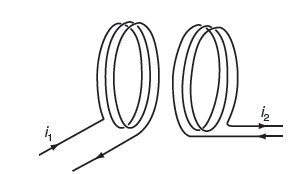
\includegraphics[width=0.5\linewidth]{imgs/19 - mutua induzione.png}
    \caption{Mutua induttanza}
    \label{fig:mutua_induttanza}
\end{figure}

La fem indotta nella bobina 1 è:
\begin{equation*}
    \epsilon_{12} = -M_{12}\frac{di_2}{dt}
\end{equation*}

Il coefficiente $M_{12}$ e $M_{21}$:
\begin{itemize}
    \item dipendono dalle proprietà geometriche del circuito
    \item vengono solitamente misurate nel circuito
    \item solo in alcuni rari casi sono facili da calcolare
\end{itemize}

La regola generale per calcolare la fem indotta in un circuito di questo tipo è:
\begin{equation}
    \epsilon_{12} = -M_{12}\frac{di_2}{dt}
\end{equation}
\begin{equation}
    \epsilon_{21} = -M_{21}\frac{di_1}{dt}
\end{equation}


\subsection{Trasformatori}
Usano la mutua induzzione per cambiare voltaggi e correnti da un circuito ad un'altro.

Solitamente si parla di primario e secondario, riferendosi al circuito 
di ingresso(primario) e al circuito di uscita(secondario).

La tensione indotta nel secondario è:
\begin{equation}
    V_s = N_s\epsilon = -N_s\frac{d\phi_B}{dt}
\end{equation}
La tensione indotta nel primario è:

\begin{equation}
    V_p = N_p\epsilon = -N_p\frac{d\phi_B}{dt}
\end{equation}

Poi spesso si utilizza semplicemente il rapporto:
\begin{equation}
    \frac{V_s}{V_p}=\frac{N_s}{N_p}
\end{equation}

E se uso le correnti, è invertito:
\begin{equation}
    \frac{I_p}{I_s}=\frac{N_s}{N_p}
\end{equation}